%-------------------------------------------------------------------------
\section{Research Plan}\label{sec:plan}
%-------------------------------------------------------------------------

%-------------------------------------------------------------------------
\subsection{Modeling of Teleoperated Robot Motion Coordination}\label{sec:plan-modeling}
%-------------------------------------------------------------------------

%-------------------------------------------------------------------------
\subsubsection{Modeling low-level motion coordination}\label{sec:plan-modeling-MP}
%-------------------------------------------------------------------------

\paragraph*{Parameterized models for low-level motion skills} Motor primitives are the building blocks of complex and goal-directed motor skills~\cite{flash2005motor}. Inspired by human motor primitives, dynamic movement primitives (DMP) were proposed for learning and producing episodic and rhythmic motions of spatial and temporal coordination~\cite{ijspeert2013dynamical}. More recently, probabilistic modeling of motion primitives has been proposed to better address demonstration regularity and variability for imitation learning~\cite{calinon2007learning,calinon2010learning}, to account for sensing uncertainty in the feedback loop control for motion reproduction~\cite{meier2016probabilistic}, and to model the temporal and spatial dependency of human-robot interaction ~\cite{maeda2017phase}. Beyond the field of imitation learning, constructing parameterized action/motion primitives has also been investigated by the robotic control \cite{fu2013bottom} and reinforcement learning (RL) communities \cite{masson2016reinforcement}. Different from motion primitives derived using Gaussian basis regression, a parameterized action is a discrete action parameterized by a real-valued vector. For example, a navigation controller is an action that is parameterized by a goal position. For a given parameter, a low-level optimal control/motion plan can be generated. Recent work proposes a RL algorithm to simultaneously learn both the optimal parameter and the low-level policy in Markov decision processes \cite{masson2016reinforcement}. However, such an episodic approach does not address spatial and temporal dependency between a set of parameterized actions. 

\paragraph*{Autonomous Motion Segmentation}



\paragraph*{Learning motion primitives from demonstrations}
The demonstrations are collected from a mobile humanoid robot controlled through various teleoperation interfaces. Standard human and robot performance metrics are used to evaluate meta performance of human-robot teleoperation system, and quantify the skill levels of novices and experts. Dynamic movement primitives (DMP) and Gaussian Mixture Model/Gaussian Mixture Regression (GMM/GMR) can used to model the motion coordination within robotic system, while Probabilistic Movement Primitives (Pro-MP) is used to model the motion coordination between robotic system and environment.

\begin{itemize}
    \item DMP
    
    \item GMM/GMR
    
    \item Pro-MP
    
\end{itemize}

\paragraph*{Learning the structure of motion primitive sets}

Human-driven classification: 

- Associate MP to robot component - hand, arm, base

- Associate MP to interface control mode

- Associate MP to motion type -- Reaching, Grasping and Locomotion Primitives

- Coupling MP of different components through shared object, task goal? 

Unsupervised learning -- Clustering MP

%-------------------------------------------------------------------------
\subsubsection{Modeling of high-level task Structure}\label{sec:plan-modeling-Plan}
%-------------------------------------------------------------------------

\paragraph{Abstract representation of robot task} The teleoperated robot tasks we consider consist of many inter-dependent procedures and complex state-action relationships. Thus, it is useful to learn abstract task structures from the demonstrations of human experts to facilitate task reasoning, decomposition, and reproduction. Previous research in robot learning has used high-level task structure representations such as Finite-State Automaton (FSA)~\cite{niekum2013semantically}, skill trees~\cite{konidaris2012robot}, and semi-Markov decision process~\cite{konidaris2018skills}. A high-level task plan can be built upon low-level motion primitives~\cite{konidaris2012robot} and symbolic representations of states and actions~\cite{konidaris2018skills}. 

We consider three abstract representations for task plan, which will lead to different task plan evaluation metrics: 


\paragraph*{Learning task plan as skill tree}


\paragraph*{Learning task plan as Semi-Markov Decision Process} Abstract task structure can be composed using symbols for actions and states. At a high-level, a teleoperated robot task structure is a semi-Markov decision process built upon the symbolic representations for the states and the actions induced state transitions. In addition, uncertainty in action can be captured with probabilistic automata. Both the action and state symbols are associated to the teleoperated robot, while the (passive) objects being manipulated are only associated with state symbols. The action symbols are abstract representation of compatible motion primitives, while the state symbols are probabilistic distributions of robot/object states learned directly from robot sensorimotor data. To relate an action to object states, we observe from the demonstrations the probabilistic distributions that describe the effects of the action. Note that the single-agent framework in~\cite{konidaris2018skills} is not sufficient to address the task complexity in multilateral teleoperation, which enables multiple teleoperators to (simultaneously) control different components of the same robotic system. Future work also needs to this framework to encompass the collaboration between a teleoperated robot and remote human collaborator. 

% Learning first order task logic


\paragraph*{Learning task plan as Probabilistic Finite-state Automaton}

% Learning high-order and temporal task logic


%-------------------------------------------------------------------------
\subsection{Comparing Teleoperation Interfaces for mobile manipulator robot}\label{sec:plan-interface}
%-------------------------------------------------------------------------

%-------------------------------------------------------------------------
\subsubsection{Platform and Preliminary work}\label{sec:plan-interface-hardware}
%-------------------------------------------------------------------------

%-------------------------------------------------------------------------
\subsubsection{Measurement metrics}\label{sec:plan-interface-metrics}
%-------------------------------------------------------------------------

%-------------------------------------------------------------------------
\subsubsection{Experiment design}\label{sec:plan-interface-exp}
%-------------------------------------------------------------------------

\paragraph{Task description}


\paragraph{Subjects}


\paragraph{Research Hypotheses}


\paragraph{Data collection and analysis}

%-------------------------------------------------------------------------
\subsection{The Development of Robot Teleoperation skill }\label{sec:plan-skill}
%-------------------------------------------------------------------------

%-------------------------------------------------------------------------
\subsubsection{Evaluating low-level motor skills}\label{sec:plan-skill-low}
%-------------------------------------------------------------------------

%-------------------------------------------------------------------------
\subsubsection{Evaluating high-level task planning}\label{sec:plan-skill-high}
%-------------------------------------------------------------------------

%-------------------------------------------------------------------------
\subsubsection{Experiment Design}\label{sec:plan-skill-exp}
%-------------------------------------------------------------------------

\paragraph{Subjects}

\paragraph{Tasks}

\paragraph{Research Hypotheses}


\paragraph{Data collection and analysis}


% Extended from the , our high-level task representation considers the effects that can only be achieved by joint human-robot action, and the effects that can be achieved by either the human or the robot. It generalizes to probabilistic transitions to capture several possible next steps given the current action and state of human (robot), and the uncertainty in dynamic task assignment. For example, a nurse may takeover the task step of the robot under certain circumstances. The abstract representation we propose is more inclusive and flexible since it encompasses the individual human/robot tasks and robot-mediated collaboration scenarios. 



% % We also observe if there exist correlation between the actions of end user and teleoperated robot to determine the coordinated motions should be modeled using interactive or independent motion primitives. 
% Here we provide more details on automata learning. Generally speaking, abstraction-based learning seeks to infer the abstract language $L$ that describes  a set of task sequences from collaborative human experts, referred to as the \emph{language of the teleoperation system}. During interactions, the autonomous system only observes finitely many instances from this language and the goal is to generalize from such observed high-level task sequences to an automaton or grammar representation of the language that may include infinitely many possible task sequences. For this task, grammatical inference (GI) \cite{de2010grammatical}, also known as automata learning, is appropriate as an abstraction-based learning mechanism. GI is a class of algorithms that generalize from a finite number of sentences to provide a grammar that describes the language, which may contain infinitely many words. As an example, consider the tele-operated robot accomplishes two tasks:  ``\textbf{P}ick up the cup (P) and \textbf{H}and it over to the nurse (H)'', and 
% ``\textbf{M}ove to the table (M), \textbf{P}ick up the cup and pla\textbf{C}e it on the shelf, and pick up the bag and hand it over to the nurse.'' These two task sequences generate a \emph{prefix}-tree, similar to a skill tree \cite{konidaris2018skills} in Fig.~\ref{fig:gi} (a) that accepts exactly two words, i.e., task sequences. Using the state merging operation \cite{de2010grammatical} in the GI algorithm, the system is able to generalize to the automaton in Fig.~\ref{fig:gi} (b), and understand it can pick and place objects infinitely often, indicated by the loop. Lastly, with another state merging, the robot learns it is able to relocate to different positions with action ``M'' (move), and can pick and place an object or hand an object over to the nurse. Using the inference algorithm, the automaton learned by GI generalizes from a skill tree to an automaton or grammar that represents a potentially infinite set of possible task decompositions and task sequences.


% \begin{figure}[t!]
%     \centering
%     \begin{subfigure}[b]{0.4\textwidth}
%         \centering
% 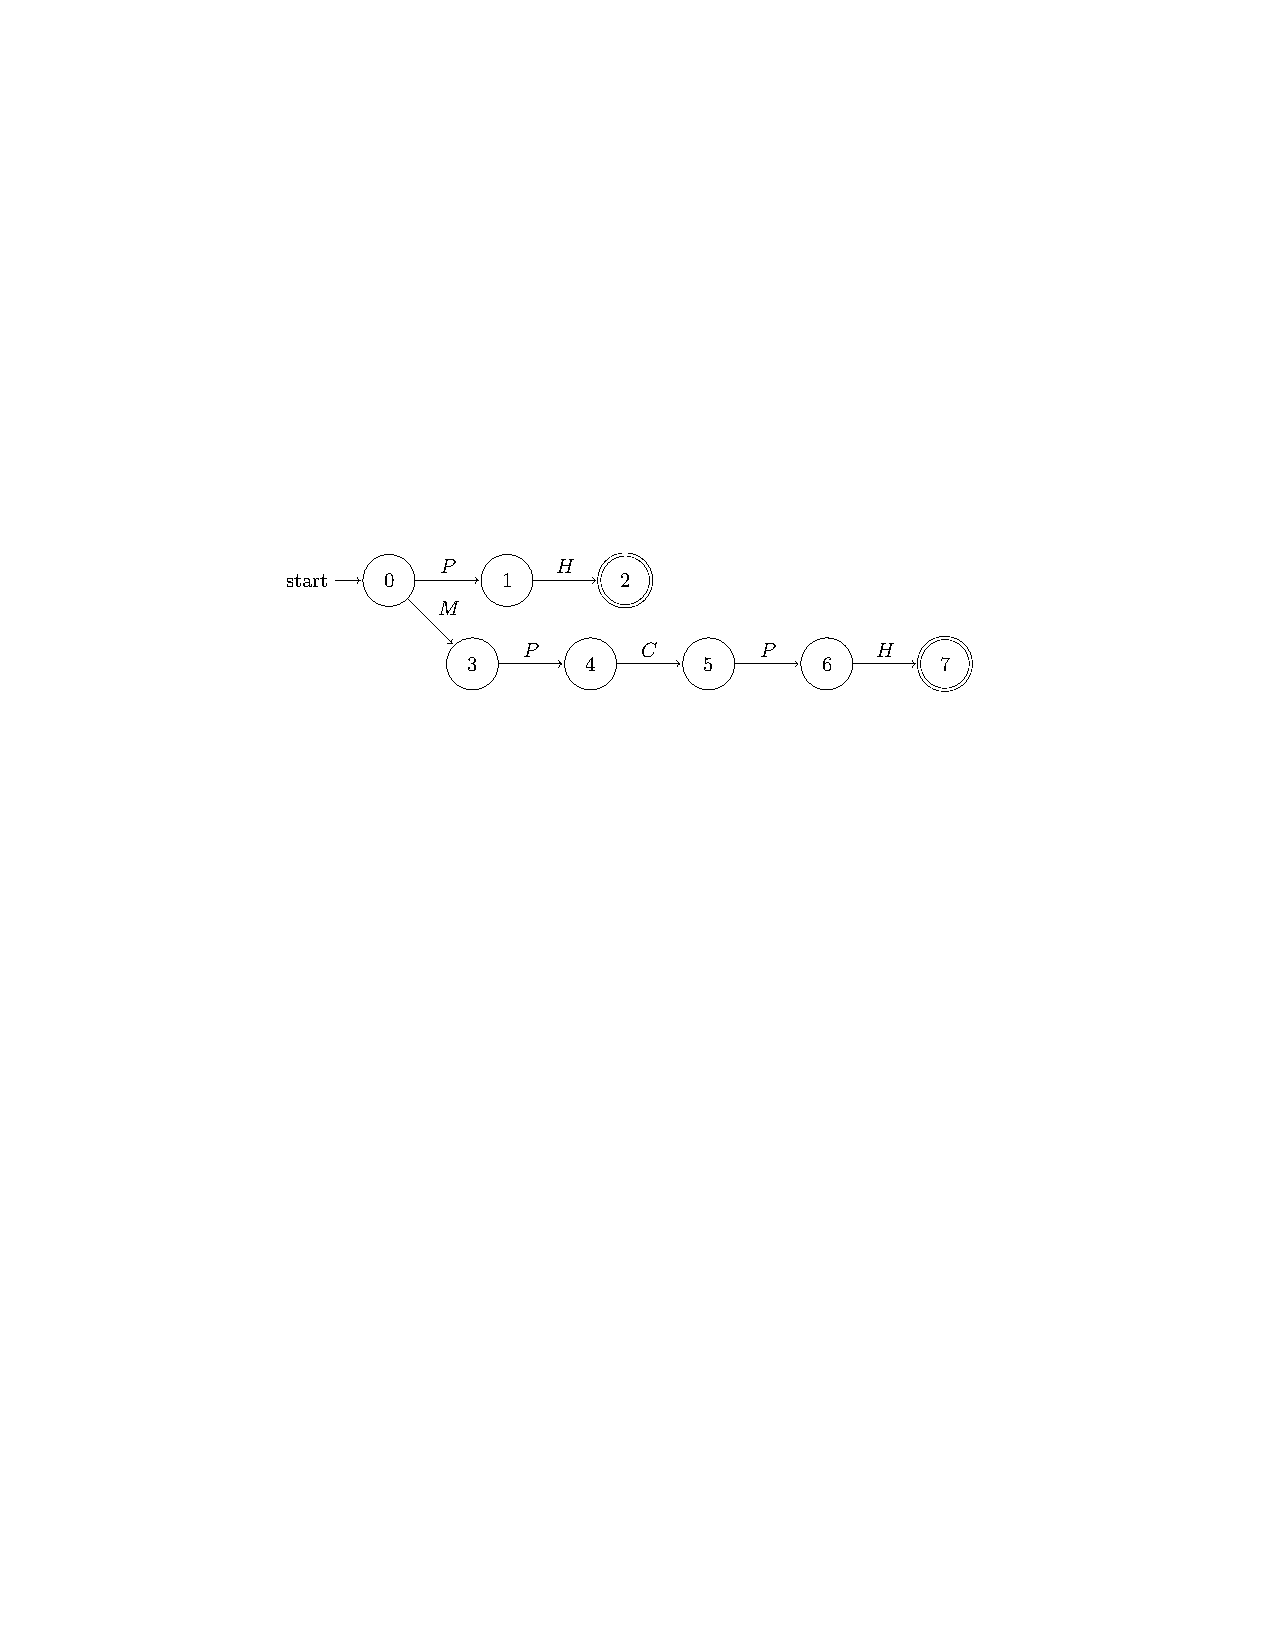
\includegraphics[width=\textwidth]{fig/original.pdf}        \caption{}
%     \end{subfigure}%
%     \begin{subfigure}[b]{0.3\textwidth}
%         \centering
% 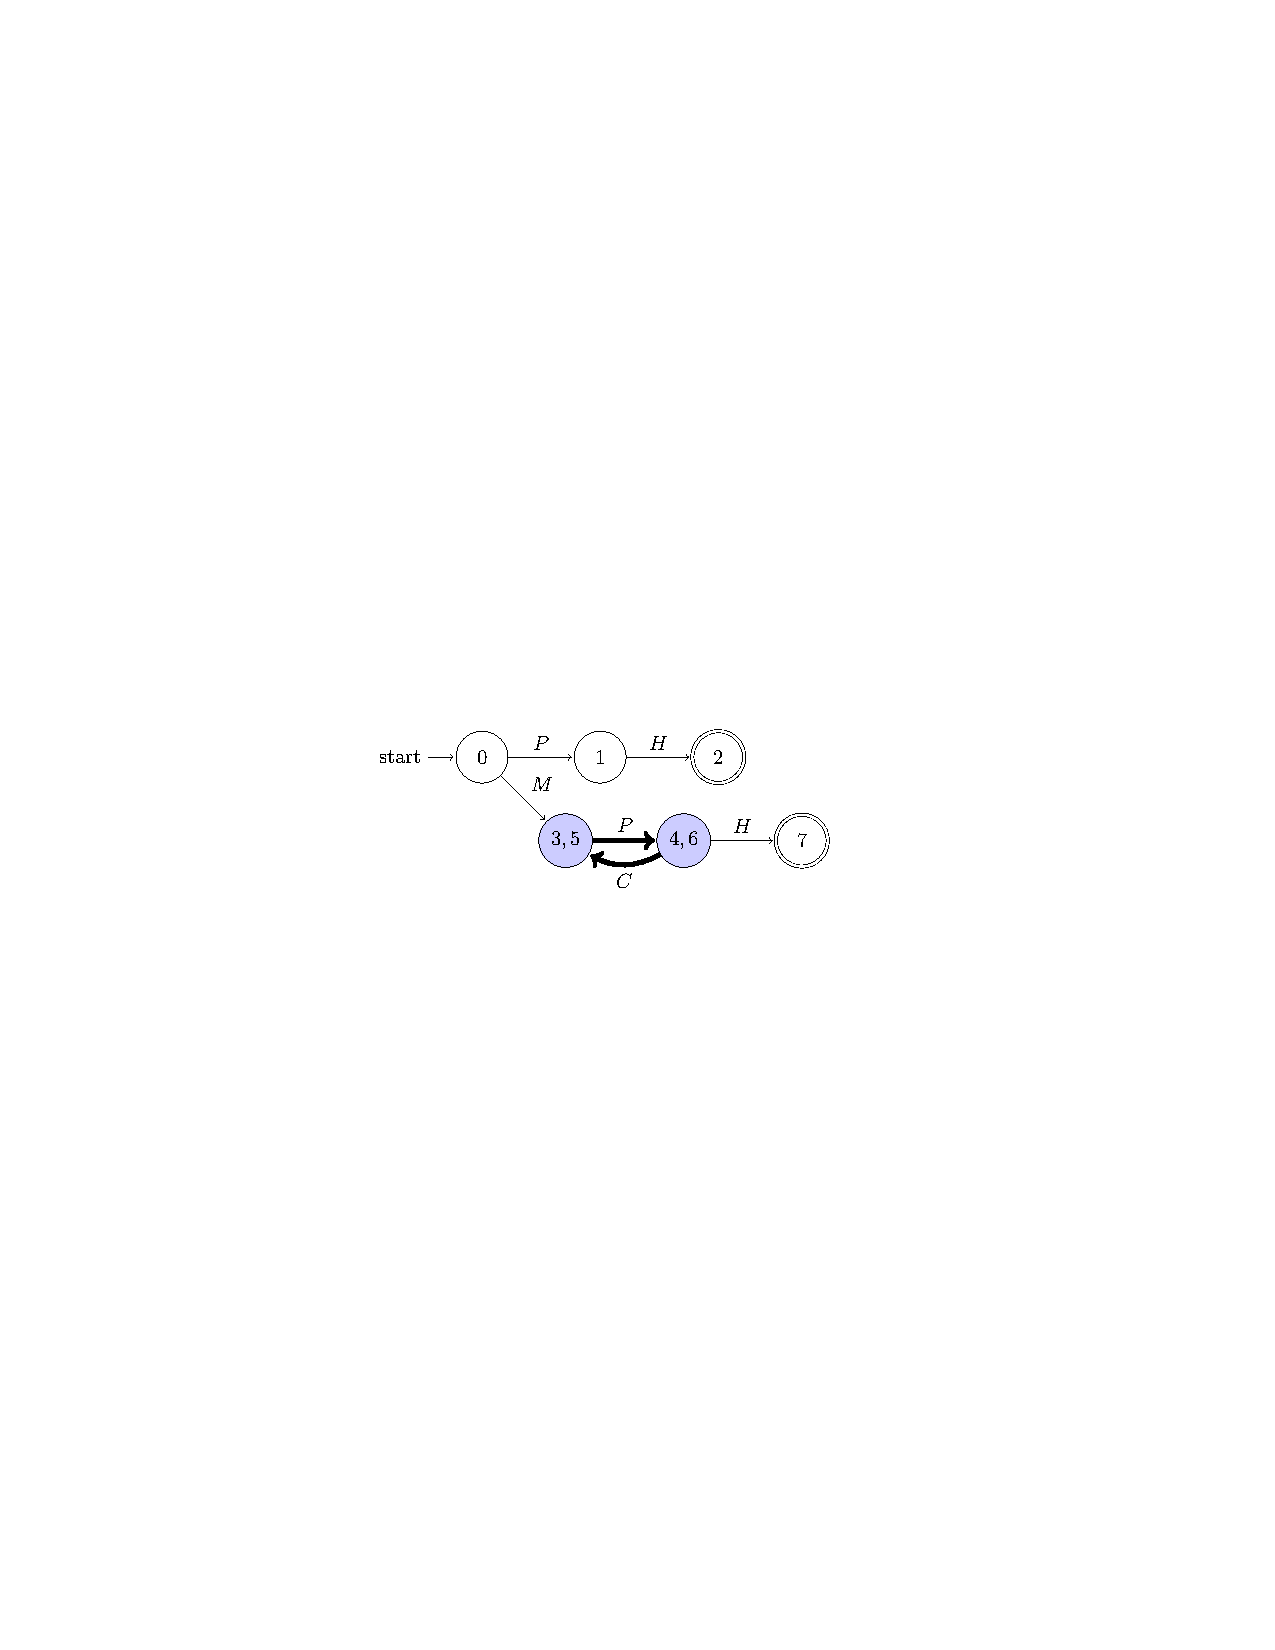
\includegraphics[width=\textwidth]{fig/merge1.pdf}         \caption{}
%     \end{subfigure}%
%     \begin{subfigure}[b]{0.28\textwidth}
%         \centering
% 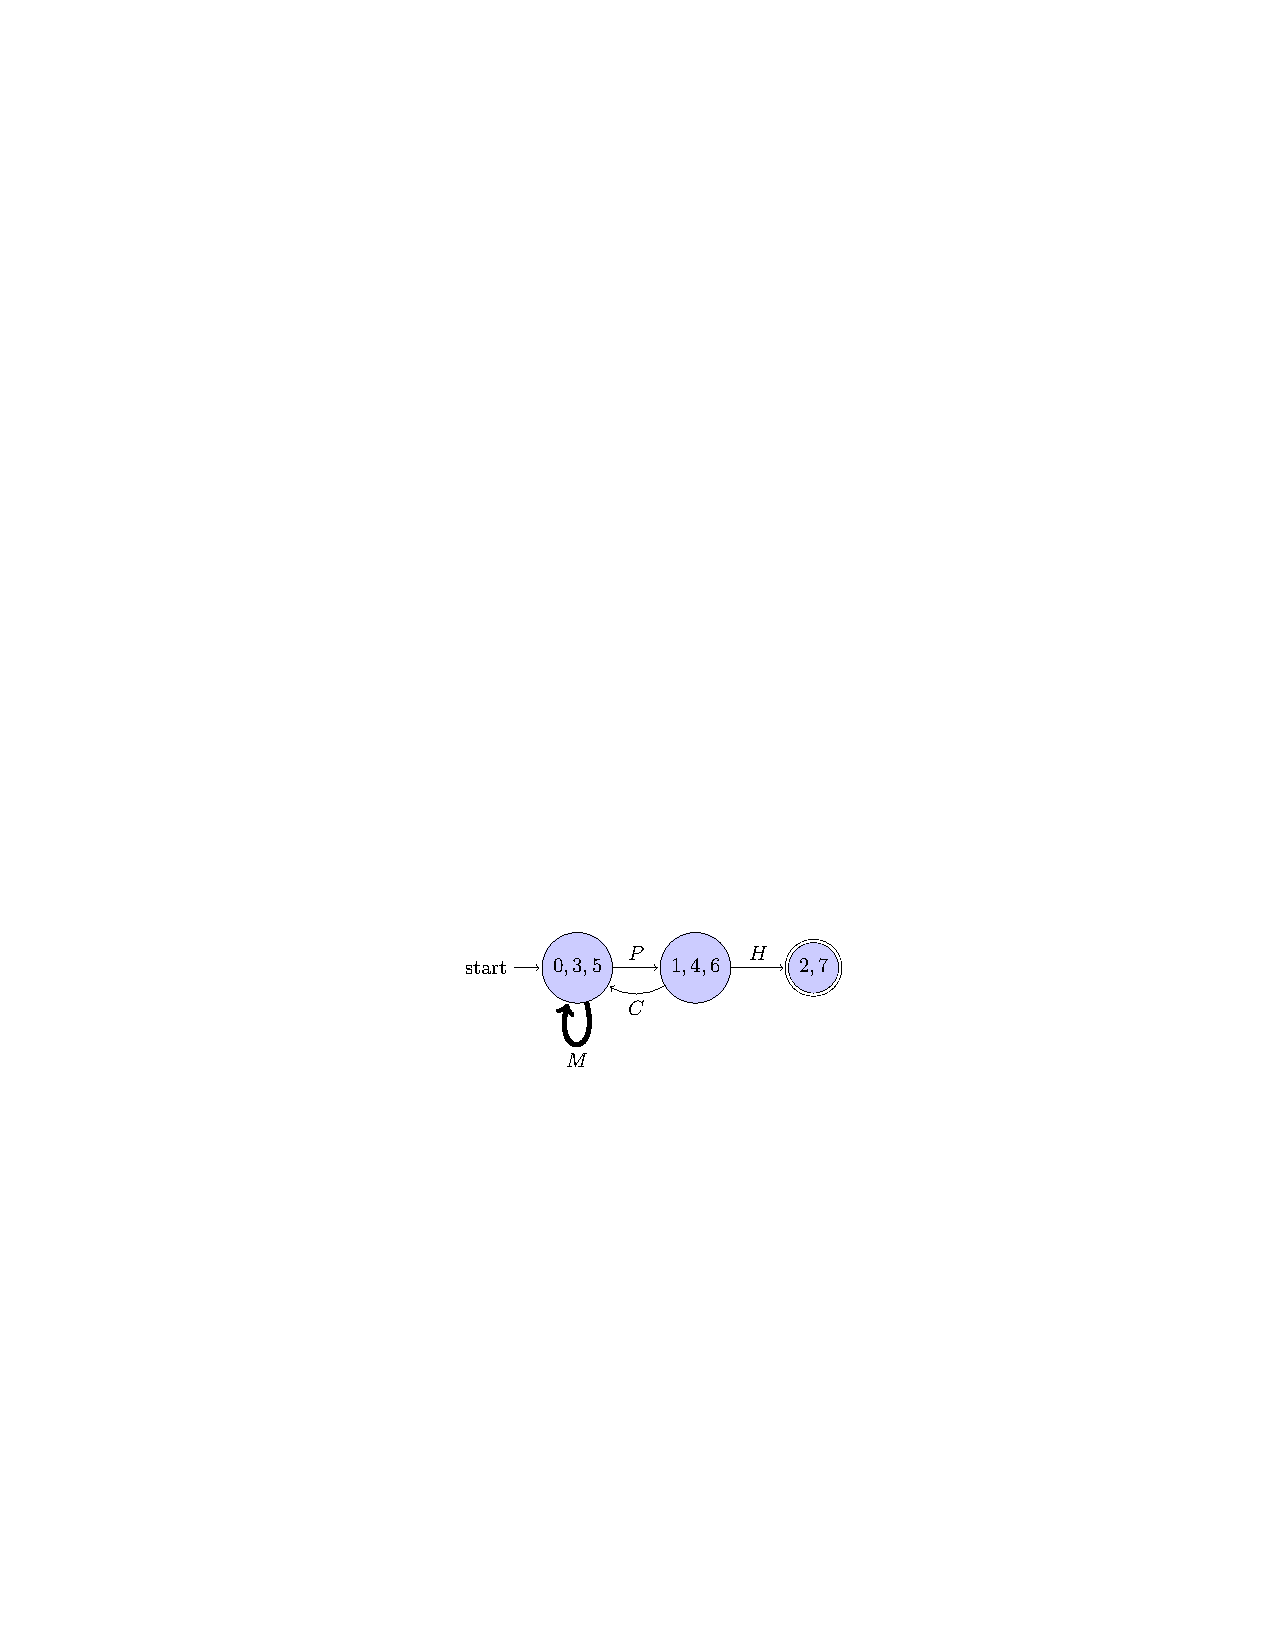
\includegraphics[width=\textwidth]{fig/merge2.pdf}     
% \caption{}\end{subfigure}
%     \caption{An illustration of the grammatical inference algorithm using state merging. (a) is the original prefix tree/skill tree. (b) generalizes (a) by merging state $3,5$ and $4,6$. (c) further generalizes (b) by merging $0,3,5$, $1,4,6$, and $2,7$. The state merging or splitting is guided by a GI algorithm selected for the target language on positive data only, or with both positive and negative data.}
%     \label{fig:gi}
% \end{figure}


% In this specific application context, we will consider several GI algorithms, including learning from positive demonstration under the assumption that actions have pairwise dependence \cite{heinz2013learning}, and the $L^\ast$ algorithm, which learns from both positive and negative demonstrations \cite{angluin1987learning}, given that negative demonstrations may be obtained from the nurses’ feedback of unreasonable behavior. We propose to learn, for three interacting agents, their individual alphabets and languages. We seperate the concern of  action synchronization, conflict, and sequencing from learning and propose to capture such constraints for collaboration and coordination through product operations between languages/automata, including but not limited to, synchronization composition and sequential composition \cite{alur2015principles,hopcroft2001introduction}. 
% For instance, synchronization will enable us to capture the dependency between the action of aiming the camera at the hand of the human nurse with the reaching motion of the manipulator.  Inference algorithms for probabilistic finite-state automata \cite{clark2004pac} \cite[Chap 12]{de2010grammatical} will further enable us to capture stochastic transitions resulting from uncertain outcomes of actions and uncertainty in task step coordination. 


% % adapt human motion coordination strategies to their remote robot surrogates.

% To meet this need, we propose to learn from novice- and expert-demonstration of the motion coordination, compare the demonstrations by their low-level motion primitive models and high-level motion plan model, to learn the features for measure the performance of human-robot teleoperation system. The demonstrations are collected from a mobile humanoid robot controlled through various teleoperation interfaces. Standard human and robot performance metrics are used to evaluate meta performance of human-robot teleoperation system, and quantify the skill levels of novices and experts. Dynamic movement primitives (DMP) and Gaussian Mixture Model/Gaussian Mixture Regression (GMM/GMR) are used to model the motion coordination within robotic system, while Probabilistic Movement Primitives (Pro-MP) is used to model the motion coordination between robotic system and environment. Novel metrics for the regularity, variability, complexity of the motion primitives are proposed as the features to characterize the low-level motor skills. Machine learning methods are used to identify the principle components and characteristic synergy in the motion primitive feature space, to compare low-level motor skills across tasks, teleoperation interfaces, and users. To model the high-level task plan, we abstract the critical robot states in motion coordination  and motion primitives for state transition to symbols, and use these symbols to construct an abstract task space graph. The costs of graph nodes and edges, which denote the abstract states and state-transition motion primitives, are assigned by weighting the teleoperator's operation efforts, efficiency, frequency and success ratio. Given the abstract motion coordination representation, we propose several optimization criteria, derived from several hypotheses of the human motion coordination strategies, and compose a reward function with unknown weighting coefficients. The weighting assignment learned from demonstrated high-level task plan can be used for evaluate and compare a teleoperator's motion coordination control strategies. 

% 





% Take the teleoperation of mobile humanoid nursing robot for instance: the motion coordination involved in patient-caring tasks includes , and may extend to the coordination of end-effectors for sensing and action. 

% skill acquisition efforts of novice worker to  

% Tele-operated robotic systems extend the physical capabilities of medical and industrial workers to perform  tasks in remote, inaccessible, and/or hazardous environments. 

% tasks that require human-level manipulation dexterity and decision-making intelligence are infeasible through autonomous control, yet can be accomplished under direct (tele)operation. To freely and efficiently control their remote surrogates, human workers need to devote significant efforts to learn the motion and perception mapping defined by the (tele)operation interface. To address this needs, we propose to investigate the physical and cognitive interactions between human workers and (tele)operation interfaces, and develop a user interface to support intuitive robot control and multi-modality cognitive augmentation. Our proposed project aims to (a) reduce the teleoperation control effort in dexterous and coordinated manipulation tasks, and to (b) facilitate novice workers to acquire the fine motor skills for operating complicate robotic systems to work on various manufacturing tasks. To this end, we propose to investigate theories and technologies that (1) Shift the boundary between direct teleoperation and autonomous control based on the physical and mental status of the operator, (2) Infer human teleoperator's contextual intent based on the knowledge of manipulation tasks and human motions, in order to automate low-level robot actions. 

% \vspace{0.5 em}

% \paragraph*{\Large Intellectual Merit}
% This project addresses how multi-modality cognitive feedback affects human motor behavior and motor learning process. Specifically, we will experimentally study in teleoperated manipulation tasks that requires simultaneous control of multiple robot components, such as loco-manipulation, bimanual coordination, arm-hand-finger coordination. For \textbf{expert workers}, we focuses on \textit{how human decision-making and task operation can be affected by single- and multi-modality cognitive feedback, and investigate methods for intuitive and integrated representation of task information and cognitive feedback}. For \textbf{novice workers}, we will focus on \textit{how multi-modality cognitive feedback affects the explicit and implicit learning of dexterous and coordinated manipulation motor skills}, as well as \textit{when and how to provide high-level/abstract cognitive feedback (e.g., verbal/text instructions, numbers, etc.) and low-level intuitive cognitive feedback (e.g., colors, shapes, sounds, tactile and forces, etc.) to facilitate the interactive and associated explicit and implicit motor learning}. Our proposed research is unique for it will develop a unified framework that integrate the model-based and model-less robot learning methodologies to reveal the underlying principles of the associated implicit and explicit human motor learning processes. The enhanced understanding of the cognitive and physical interactions between human worker and teleoperation interfaces further leads to novel techniques for user-adaptive cognitive augmentation and decision-making assistance, which leverages ``cloud wisdom'' and adjust the human-robot control efforts based on a human worker's intents, physical/mental states, and skill level. 

% % to robot learning that acquire motion and task knowledge through  (e.g., reinforcement learning with explicit reward function v.s. learning through convolutional neural network). Inspired by how human can develop situational awareness and motor skills through intuitive and abstract cognitive feedback and augmentation, we will further develop novel robot teaching methodologies for that leverage human-guided robot interactions with environments and demonstrations/critiques from human teachers. 

